\subsection{Gaussian fit for spectral lines}
In order to accurately determine the wavelength of the different spectral lines, every peak was identified from the clean data and then fitted by a Gaussian\cite{Gaussian} function. The formula used is described here:

\begin{equation} \label{eqn}
	f(x)=A\cdot \mathrm{e}_{}^{\frac{-1}{2}\cdot\left( \frac{x-b}{c} \right)^{2}}
\end{equation}

\begin{itemize}
    \item A describes the amplitude of the curve (maximum intensity)
    \item b describes the middle position of the curve (corresponds to peak wavelength)
    \item c describes the standard deviation of the curve
\end{itemize}

After every peak is identified in the clean data, the Gaussian fit function was used in Matlab as per below for every one of the 8 spectral lines identified in each of the 4 spectra. The result for the first spectral line of the first data-set is plotted in \textbf{Figure \ref{fig:Figure 12}}. The rest of the Gaussian fit plots can be found in the Appendix[\ref{fig:Figure 13}]. Also general information about the average values of the peaks obtained are in the \textbf{Table \ref{tab:table2}} and\textbf{ Table \ref{tab:table3}} below. There is a general error of 0.02 nm in the wavelength values due to the sample resolution of the wavelengths, or distance between points in the x-axis being 0.02 nm.

\begin{lstlisting}
    ft = fittype( 'gauss1' );
    opts = fitoptions( 'Method', 'NonlinearLeastSquares' );
    [fitresult, gof] = fit( xData, yData, ft, opts );
\end{lstlisting}

\begin{figure}[H]
    \centering
    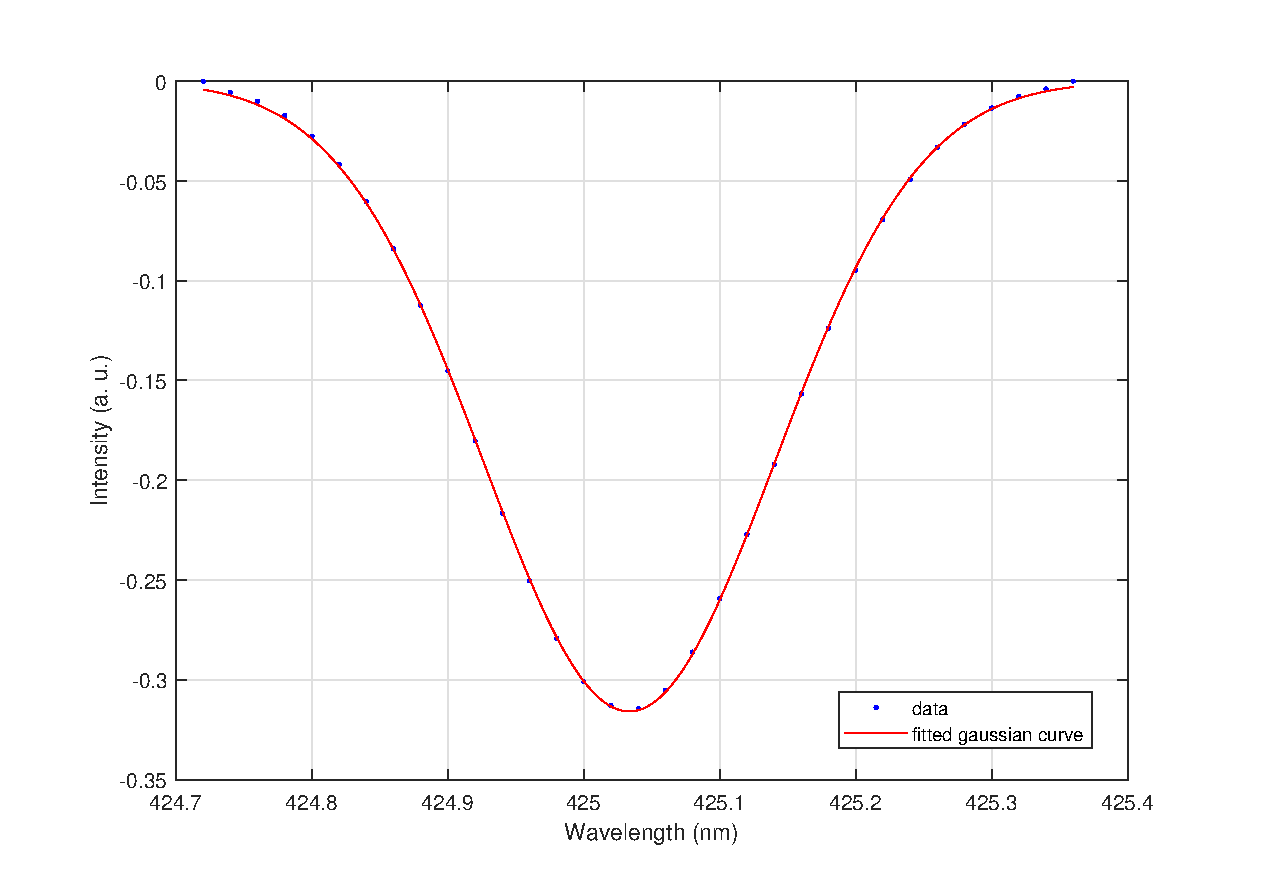
\includegraphics[width = 1\textwidth ]{figures/gauss_1.eps}
    \caption{Gaussian fit for spectral line 1 of spectrum 1 }
    \label{fig:Figure 12}
\end{figure}


\begin{table}[H]
    \centering
    \caption{Average maximum intensity of the peaks}
    \begin{tabular}{|c|c|c|c|c|c|c|c|c|}
    \centering
    \textbf{}   & \textbf{Line 1} & \textbf{Line 2} &  \textbf{Line 3} & \textbf{Line 4} & \textbf{Line 5} & \textbf{Line 6} & \textbf{Line 7} & \textbf{Line 8}\\ \hline \hline
    Spectrum 1   & -0.3158    & -0.3968    & -0.2430 & -0.1282  & -0.0961 & -0.0069 & 0.0234 & -0.0686 \\ \hline   
    Spectrum 2   & -0.3158    & -0.3977    & -0.2430 & -0.1282  & -0.0961 & -0.0069 & 0.0232 & -0.0685\\ \hline
    Spectrum 3   & -0.3157    & -0.3976    & -0.2429 & -0.1282  & -0.0960 & -0.0068 & 0.0233 & -0.0685\\ \hline
    Spectrum 4   & -0.3158    & -0.3981    & -0.2430 & -0.1281  & -0.0961 & -0.0070 & 0.0233 & -0.0684\\ \hline
   \textbf{Average}   & \textbf{-0.3158}    & \textbf{-0.3976}    & \textbf{-0.2430} & \textbf{-0.1282}  & \textbf{-0.0961} &\textbf{ -0.0069} & \textbf{0.0233} & \textbf{-0.0685}
    \end{tabular}
    \label{tab:table2}
\end{table}

\begin{table}[H]
    \centering
    \caption{Average wavelength of the Gaussian peak maximum (nm), with error tolerance of $\pm 0.02 nm$}
    \begin{tabular}{|c|c|c|c|c|c|c|c|c|}
    \centering
    \textbf{}   & \textbf{Line 1} & \textbf{Line 2} &  \textbf{Line 3} & \textbf{Line 4} & \textbf{Line 5} & \textbf{Line 6} & \textbf{Line 7} & \textbf{Line 8}\\ \hline \hline
    Spectrum 1   & 425.02    & 426.04    & 427.18 & 428.24  & 440.20 & 446.76 & 523.22 & 583.72 \\ \hline   
    Spectrum 2   & 425.04    & 426.06    & 427.18 & 428.24  & 440.22 & 446.78 & 523.24 & 583.74\\ \hline
    Spectrum 3   & 425.06    & 426.08    & 427.20 & 428.26  & 440.24 & 446.80 & 523.24 & 583.76\\ \hline
    Spectrum 4   & 425.08    & 426.08    & 427.22 & 428.28  & 440.24 & 446.80 & 523.26 & 583.78\\ \hline
    \textbf{Average}     & \textbf{425.06}    & \textbf{426.06}    & \textbf{427.20} & \textbf{428.26}  & \textbf{440.22} & \textbf{446.80} & \textbf{523.24 }& \textbf{583.76}
    \end{tabular}
    \label{tab:table3}
\end{table}

\subsection{Element determination for spectral lines}
After determining the average peak wavelengths of each spectral line and their intensity, 4 of those lines towards the lower end of the spectrum were selected and compared against an online database from the website of the National Institute of Standards and Technology (\textbf{NIST})\cite{NIST} (https://www.nist.gov/pml/atomic-spectra-database). For this purpose, a companion script written in Python was made to connect to the API of NIST, query and download the required data.
The script parses command-line data and generates a URL that then uses to extract data regarding the specific wavelengths in the range, element names and relative intensities of the spectral lines in question and saves the data to csv files to be read by matlab. Information on how to use it can be found in comments inside the script.
\begin{lstlisting}
API_NIST_v3.py

# Example usage:
#
# python.exe .\API_NIST_v3.py 426.5 data --element Fe --n 10 --low_w 425 --high_w 584 --ion_num 1 2 --min_intensity 10
\end{lstlisting}
After the query is complete, another matlab function loads the data (if it wasn't saved already), cleans it up, eliminating repeated rows, and identifies the most likely element according to the given wavelengths and intensities. This is done by looping over all spectral lines in the database and calculating the error by calculating the square difference between those values and the averages of the spectral lines' wavelengths calculated earlier.

\begin{lstlisting}
% Loop over each element in NIST_data_unique
    for i = 1:size(NIST_data_unique, 1)
        % Calculate the error between the current element and x_peaks/x_peaks_max
        error1 = sum((wavelengths(i) - x_peaks).^2);
        % error2 = sum((intensities(i) - x_peaks_max).^2);
        error = error1 + error2;
        
        % Update the closest match if the error is smaller than the current minimum
        if error < min_error
            min_error = error;
            matched_index = i;
        end
    end
    matched_element = NIST_data_unique(matched_index, 1);
\end{lstlisting}

As a result it returns the element with the lowest error value.
In this particular case, the identified element was \textbf{Chromium (Cr)}, with a match error score of: 5.7832, although other elements came close, such as Iron (Fe) with a score of 5.7886, and Actinium (Ac), with a score of 5.7877, despite being unlikely due to it being a rare metal.
